\section{Sauvegarde}
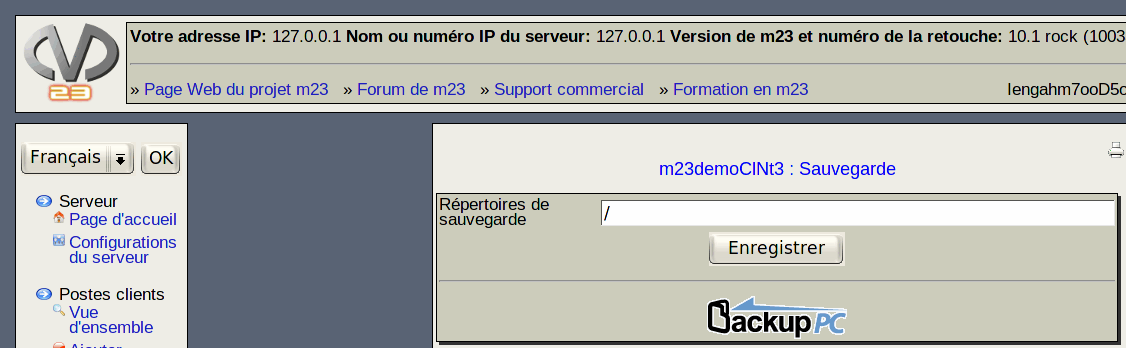
\includegraphics[scale=0.4]{/mdk/doc/manual/screenshots/fr/client_backup.png} \\
Dans ce dialogue, vous pouvez indiquer tous les r\'epertoires du poste client que vous voudriez sauvegarder. Entrez ces r\'epertoires, s\'epar\'es par des virgules, dans le champ de saisie \textit{$\ll$R�pertoires de sauvegarde$\gg$} et puis, cliquez sur \textit{$\ll$Enregistrer$\gg$}.\\
La vraie sauvegarde sera ex\'ecut\'ee par le programme BackupPC, que vous pouvez d\'emarrer par un clic sur l'ic\^one. Dans l'interface graphique de BackupPC, vous avez acc\`es \`a des fonctions de sauvegarde additionnelles.\\
